\chapter{Introduction}\label{sec:matrices}


This proposal is about simple dynamical networks, with dynamics
that are described either by a stochastic rate equation
%
\begin{align}
  \frac{d}{dt}\mathbf{p} \quad &= \quad -\mathbf{K} \mathbf{p} \\
  \mathbf{K} \quad &\equiv \quad \textrm{diag}\{ \gamma_n \} \ \ +\ \ \textrm{offdiag}\{ -w_{nm} \} \\
  \mathbf{p} \quad &\equiv \quad \textrm{vector}\{ p_n \}
\end{align}
%
by the Schr\"{o}dinger equation:
%
\begin{align}
  \frac{d}{dt}\psi \quad &= \quad -i \mathcal{H}\psi \\
  \mathbf{\psi} \quad &\equiv \quad \textrm{vector}\{ \psi_n \}
\end{align}
%
or by Newton's second law:
%
\begin{align}
  \frac{d^2}{dt^2}\mathbf{q} \quad &= \quad -\mathbf{K} \mathbf{q} \\
  \mathbf{q} \quad &\equiv \quad \textrm{vector}\{ q_n \}
\end{align}
%

All of these equations 
involve {\rm real} matrices that describe {\em disordered} 
one- two- and quasi-one- dimensional structures. The elements of
the matrices may be randomized directly to simulate disorder, or they
could depend on a random spatial distribution of sites. For example, in 
part of the work we use a transition rate matrix defined by
%
\begin{align}
w_{nm} \quad = \quad w_0 \eexp{-\epsilon_{nm}}B(x_n-x_m)
\end{align}
%
where $\epsilon_{nm}$ represents activation energies required for transitions,
and $B(r)$ defines a dependence on the distance between sites. The matrix
that consists of these distances is called a euclidean distance matrix, 
a class of matrices that is widely researched both in physics and in mathematics 
\cite{skipetrov_eigenvalue_2011, goetschy_non-hermitian_2011,mezard_spectra_1999, bogomolny_spectral_2003}.

In general, these matrices 
are of physical interest in various applications including:

\begin{enumerate}[label={\Alph*.}]
\item Resistor networks / random walk / hopping 
\item Rate equations / relaxation processes 
\item Mechanical elastic vibrations (``balls and springs'')
\item Electrical R-L-C circuits.
\item Hermitian quantum dynamics with time-reversal symmetry. 
\item Non-Hermitian quantum dynamics with any anti-unitary symmetry. 
\end{enumerate}

In particular we note that the Mott impurity hopping problem 
\cite{miller_impurity_1960,movaghar_theory_1981}
belongs to category A. The problem of Sinai spreading (``random 
walk in random environment'')
\cite{sinai_limiting_1983,bouchaud_anomalous_1990}
belongs to category B.
The theory of heat conduction 
\cite{nagel_normal-mode_1981,schirmacher_analogies_1992,
amir_localization_2010,amir_mean-field_2008,tong_wave_1999}
belongs to category C. 
Studies of wave-packet dynamics\cite{izrailev_evolution_1997,cohen_wave_2000} belong to E, and 
in particular the recent interest in systems that are described by 
a non-Hermitian PT symmetric hamiltonian
\cite{bender_exactly_2008,mannheim_astrophysical_2012,jin_physical_2011,zheng_heat_2011}
 belongs to category F.

In the present proposal we would like to emphasize the 
implications of {\em sparsity}, meaning extreme disorder 
due to log-wide distribution of matrix elements
\cite{rodgers_density_1988,biroli_single_1999,
fortin_asymptotic_2005,metz_localization_2010,
cohen_energy_2012,stotland_semilinear_2009}. 
We note that {\em localization} and {\em percolation} are strongly 
related aspects in the analysis of transport in such systems. 


The real matrices that we consider can be characterized 
by several properties, which we list here in order of increasing 
complexity, and further elaborate below:

\begin{enumerate}
\item Symmetry.
\item Non-negativity.
\item Conservation.
\item Detailed balance.
\item Frustration.
\item Diagonal disorder.
\item Broken reality.
\end{enumerate}

The eignevalues of a real matrix are the roots of a characteristic 
polynomial that has real coefficients. Hence the spectrum consists 
of real eigenvalues, and optionally also pair of complex-conjugate 
values. 

By ``non-negativity'' we mean that all eigenvalues are real and 
non-negative: for example in the context of rate equations it means 
that all the eigen-modes are decaying except the steady state 
that has zero eigenvalue. 

By ``Broken-reality'' we mean that some of the eigenvalues  
become complex: in particular this might happen 
as we vary some control parameter. The studies of ``PT broken symmetry'' 
provide an example for such scenario. One should realize that  
a complex eigen-state that is associated with a complex eigenvalue 
has a {\em lower} symmetry than that of the Hamiltonian.

It is most common to consider a {\em symmetric} matrix. 
All the eigenvalues of such matrix are real. 
Such matrices appear in Hamiltonian dynamics 
if the system has anti-unitary (say time reversal) symmetry.  

A special sub-class of symmetric matrices consists of those 
that are both non-negative and conserving. Such matrices
can be regarded as describing a ``resistor network''.
They have positive off-diagonal elements that describes 
the connectors, while their diagonal elements are determined 
such that the probability (or the charge) is conserved. Namely 

%gamma_n \equiv ... = ... 
%
\begin{align}\label{eq:zero_sum}
\gamma_n \ \ \equiv \ \ \sum_{m\ne n} w_{mn}
\end{align}
%

The eigenvalues of a non-negative conserving symmetric matrix, 
are all non-negative and represent decay or diffusion modes of the network. 
Only the ergodic state is non-decaying with zero eigenvalue.   

More generally rate-equation matrices are non-negative, conserving, 
but non-symmetric. Hence they have real positive eigenvalues 
that are associated with the decay modes of the system, 
and a zero mode that describes the steady state.  

It should be realized that the dynamics that is generated 
by  a ``resistor network'' matrix (``infinite temperature'') 
resembles diffusion or percolation process, while that of 
a ``finite temperature'' network (non-symmetric matrix) has to 
do with Sinai spreading (as discussed in \autoref{sec:sinai}).  

A special sub-class of conserving non-negative matrices 
are {\em detailed-balanced}. See \autoref{sec:detailed_balance} for precise definition. 
Hence there is a simple "canonical" expression for their 
ground state. More generally the system might be frustrated 
hence the "non-equilibrium" steady state might carry current.

The matrix that describes a system that is composed 
of balls connected by springs is similar to that of a 
rate equation, but has diagonal elements that might contain 
an additional contribution that reflects a pinning potential 
that attaches each ball to a fixed location.   



%%%%%%%%%%%%%%%%%%%%%%%%%%%%%%%%%%%%%%%%%%%%%%%%%%%%%%%
\section{Diffusion and sub-diffusion}


We define a diffusion coefficient $D$, either by the spreading $S(t)$
or by the survival probability $\mathcal{P}(t)$:
%
\begin{align}
D\ \ &\sim\ \ \frac{S(t)}{t}  \quad \textrm{as }\ t\rightarrow\infty \\
\mathcal{P}(t)\ \ &\sim\ \ (Dt)^{-d/2}
\end{align}
%
For a stochastic network, $S(t)$ can be studied via resistor network 
calculations. $\mathcal{P}(t)$ is the Laplace transform of the 
eigenvalue density, hence it can be deduced from the spectral properties of the 
system. 
%


%%%%%%%%%%%%%%%%%%%%%%%%%%%%%%%%%%%%%%%%%%%%%%%%%%%%%%%
\section{The Anderson localization}\label{sec:anderson}

 %following the seminal work of Anderson \cite{anderson_absence_1958,markos_numerical_2006},
By adding uncorrelated disorder to crystals, some of the electronic eigenstates 
localize\cite{anderson_absence_1958,mott_mobility_1987,thouless_electrons_1974}. In  $d=1$ all the states are localized, as well as in $d=2$ real matrices 
(i.e.\ without magnetic field). In $d=3$ and higher, if the disorder
is small enough, a mobility edge divides the spectrum to localized states \emph{below} the edge and 
de-localized states \emph{above} the edge. In the case of an energy band, i.e.\ $\lambda\in [-\lambda_c,\lambda_c]$,
the states at the end of the band will be localized, while those in the middle
will be de-localized meaning that there are two mobility edges,
where the only de-localized states are those \emph{between} the edges.


The picture in phonon vibrations is somewhat different
\cite{tong_wave_1999,reuveni_anomalies_2010,granek_fractons_2005,ishii_localization_1973,lepri_thermal_2001,kantelhardt_extended_1998,amir_localization_2010}. 
In a conserving
system, as defined earlier, there is always one de-localized ergodic mode with $\lambda=0$.
If we are dealing with a non-negative matrix such as in rate equations, 
then $\lambda \in [0,\lambda_c]$, and the de-localized ergodic mode
sits on the lower edge of the spectrum. This means that either that the localization 
length diverges as $\lambda\rightarrow 0$, or that the system is de-localized for
$\lambda\rightarrow 0$.


At first sight those pictures seem incompatible. But the fact 
of the matter is, that the spectrum of the phonon vibrations
can be thought of as the upper half of an electron band, as caricatured in \autoref{fig:bands}.



\begin{figure}
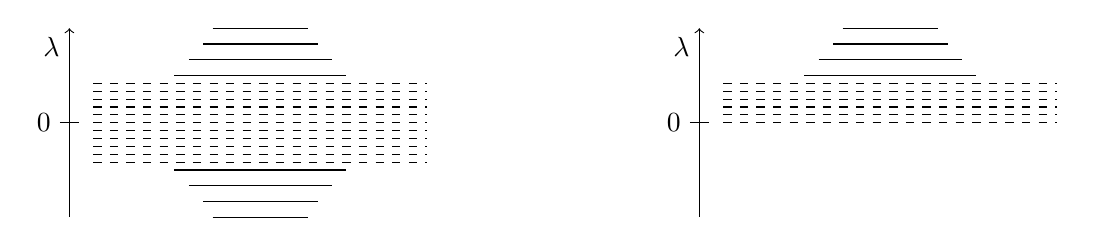
\begin{tikzpicture}[x=\textwidth/20,y=0.2cm]

\draw[black] (-1,6) --(1,6);
\draw[black] (-1.2,5) --(1.2,5);
\draw[black] (-1.5,4) --(1.5,4);
\draw[black] (-1.8,3) --(1.8,3);
%draw[black,dashed] (-3,6) rectangle (3,2);

\foreach \y in {-5,...,5}
        \draw[dashed] (-3.5,\y/2)  -- (3.5,\y/2);

\draw[black] (-1.8,-3) --(1.8,-3);
\draw[black] (-1.5,-4) --(1.5,-4);
\draw[black] (-1.2,-5) --(1.2,-5);
\draw[black] (-1,-6) --(1,-6);
%axis:
\draw[->] (-4,-6) --(-4,6) node [pos=0.9,left] {$\lambda$};
\draw (-4-0.2,0) -- (-4+0.2,0) node[left] {$0\ \ $   };



%%%%%%%%%%%%%%%
%% RIGHT SIDE, dirty copy-paste

\draw[black,xshift=8cm] (-1,6) --(1,6);
\draw[black,xshift=8cm] (-1.2,5) --(1.2,5);
\draw[black,xshift=8cm] (-1.5,4) --(1.5,4);
\draw[black,xshift=8cm] (-1.8,3) --(1.8,3);
%draw[black,dashed] (-3,6) rectangle (3,2);

\foreach \y in {-5,...,5}
        \draw[dashed,xshift=8cm] (-3.5,\y/2)  -- (3.5,\y/2);

\draw[black,xshift=8cm] (-1.8,-3) --(1.8,-3);
\draw[black,xshift=8cm] (-1.5,-4) --(1.5,-4);
\draw[black,xshift=8cm] (-1.2,-5) --(1.2,-5);
\draw[black,xshift=8cm] (-1,-6) --(1,-6);
%axis:
\draw[->,xshift=8cm] (-4,-6) --(-4,6) node [pos=0.9,left] {$\lambda$};
\draw[xshift=8cm] (-4-0.2,0) -- (-4+0.2,0) node[left] {$0\ \ $   };


\fill[white,xshift=8cm]  (-3.9,-0.1) rectangle (4,-6.2);
\end{tikzpicture}
\caption{The eigenstates in a $d=3$ disordered system. The full lines represent localized modes, 
 their width representing the localization length.
  The dashed lines are the de-localized modes. On the left for a banded
  spectrum, on the right for a banded non-negative spectrum  }
     \label{fig:bands}
\end{figure}




There are several routines used to distinguish between exponentially localized and delocalized modes.
The most straight forward one seems to be the participation number (PN) 
\cite{edwards_numerical_1972}, which is defined by its inverse:
%
\begin{align}
PN^{-1} \ =\ \sum_i p_i^2
\end{align}
where $p_i$ is the probability to be in a specific site, equal to $|\psi_i|^2$ 
for a quantum wave function. For a fully extended mode $PN\sim N$, while for a state
occupying only one site $PN = 1 $.


Another idea called Thouless curvature or Thouless conductance 
\cite{edwards_numerical_1972,thouless_electrons_1974,braun_level_1997}, is based
on the idea that localized eigenmodes are almost not sensitive to boundary conditions. We apply a 
phase change $\phi$ across the boundary, (due to gauge invariance the specific spot is irrelevant),
and check the resulting change in the eigenvalues. 
In an ordered system with extended modes, $\phi=\pi$ will cause an energy
shift larger than the level spacing. 
Using perturbation theory on Kubo's equation \cite{kubo_statistical-mechanical_1957},
Thouless defined a conductance that is proportional to the diffusion: 
\begin{align}\label{eq:thouless}
\bra g_T\ket  \equiv \pi \frac{\bra \left|\left. \frac{\partial ^2 E^{(n)}}{\partial \phi^2}\right|_{\phi\rightarrow 0}\right|\ket}{\Delta}
\end{align}
where $\Delta$ is the level spacing.




%%%%%%%%%%%%%%%%%%%%%%%%%%%%%%%%%%%%%%%%%%%%
\section{Modeling quantum diffusion with resistor networks}

%In past work \cite{cohen_wave_2000} 

In a model described by a Hamiltonian 
%
\begin{align}
\mathcal{H} = \textrm{diag}{E_n} + \epsilon {V_{nm}}
\end{align}
%
according to the first step of perturbation theory (Fermi's golden rule),
for very short time the transition probability is:
%
\begin{align}
 p(n, n_0)\ =\ \left| \epsilon \bra n| V |n_0\ket t\right|^2 \ = \ \epsilon^2 t^2\left| \bra n| V |n_0\ket \right|^2
\end{align}
%
This suggests that for some short time scale, the ballistic behavior
of the system is related to the conductivity of the rate equation $G_{nm} = \left| \bra n| V |n_0\ket \right|^2$.





%%%%%%%%%%%%%%%%%%%%%%%%%%%%%%%%%%%%%%%%%%%%%%%
\section{Heat conductance}\label{sec:heat}

One can take one of our suggested models, and couple each end to a different heat bath.
Assuming white-noise baths at sufficient temperature, the total heat conductance of the sample is defined by:
\begin{align}
G = \int_0^\infty \rho(\lambda) g(\lambda) d\lambda
\end{align}
where $\rho(\omega)$ is the density of states, and $g(\lambda)$ is 
a transmission coefficient for a phonon at energy $\lambda$.
$g(\lambda)$ is highly affected by the localization length of this mode\cite{tong_wave_1999}.
The high frequency eigenmodes are strongly localized, hence only the
lower part of the spectrum contributes to the heat flux. Based on this idea,
the heat flux can be estimated \cite{lepri_thermal_2001,lepri_thermal_2003,bodyfelt_unpub},
by the number of wide modes times their localization length.

 
Many one-dimensional models 
\cite{narayan_anomalous_2002,dhar_heat_2001,lepri_anomalous_1998,savin_heat_2002} 
exhibit sample size scaling of the form
%
\begin{align}
g(\lambda)    &\propto L^\alpha
\end{align}

There is an open debate regarding $d=1$ systems,
with momentum conservation or pinning potentials, 
with results such as $\alpha=1/3$,$\alpha=2/5$ or neither
\cite{narayan_anomalous_2002,delfini_comment_2008,dhar_dhar_2008,wang_power-law_2011,basile_momentum_2006}.
For several systems it has been shown that $\alpha$ depends on some tunable potential \cite{tong_wave_1999},
and it also depends on the spectrum of the baths \cite{dhar_heat_2001}.




%%%%%%%%%%%%%%%%%%%%%%%%%%%%%%%%%%%%%%%%%%%%%%%%%%%%%%
\section{Covariance matrix formalism}

We define the ($2N\times 2N$) covariance matrix as:
\begin{align}
\mathbf{C} \ &=\ \langle \vec{z}\otimes \vec{z}\rangle \ =\ 
              \begin{pmatrix} 
                C^{qq} & C^{qp} \\
                C^{pq} & C^{pp}
            \end{pmatrix}
\\
\vec{z} &= (q_1,\ldots q_N, p_1,\ldots p_N)^\intercal
\end{align}


In the NESS (non equilibrium steady state), $\mathbf{C}$ 
is the solution of the following Lyapunov equation 
\cite{bodyfelt_unpub,zheng,zheng_heat_2011,bhatia_how_1997,dhar_heat_2008,rieder_properties_1967,*nakazawa_energy_1968,*matsuda_localization_1970}:
%
\begin{align}
&\mathbf{Z}\mathbf{C} + \mathbf{C}\mathbf{Z}^\intercal + (T_R\mathbf{Y}^R+T_L\mathbf{Y}^L) \ =\  0\\
\mathbf{Z} &= 
              \begin{pmatrix} 
                \mathbf{0} & \mathbf{1} \\
                \mathbf{K} & \mathbf{0} 
              \end{pmatrix} -(\mathbf{Y}^R+\mathbf{Y}^L)
\end{align}
%
Where $\mathbf{Y}^{L,R}$ are diagonal matrices that couple
the system to heat baths at temperatures $T_R$ and $T_L$ accordingly.
%
The local temperature and conductance are defined as
\begin{align}
T_n &= \langle p_n^2 \rangle \ = \ C^{pp}_{n} \\
%J_n &= \sum_l\frac{1}{m}\left\langle \left(\vec{p}^{\intercal} \mathbf{K} \vec{q}\right)_{nl} \right\rangle
J_n &= \sum_{i\ge n}\sum_{j<n} \frac{1}{m}\left\langle \left(p_i K_{ij} q_j\right) \right\rangle 
= \sum_{i\ge n}\sum_{j<n}\frac{1}{m}  K_{ij} C^{pq}_{ij}
\end{align}

This relates the incoming and outgoing flux of heat 
to the local temperatures. This idea is very similar
to the familiar resistor network calculation based on Kirchoff's equation, with 
heat flux replacing current, and local temperature replacing voltage. 
 

%%%%%%%%%%%%%%%%%%%%%%%%%%%%%%%%%%%%%%%%%%%%%%%%%%%%%
\begin{comment}
\section{Banded matrices spectrum}


For wide bandwidth and uncorrelated matrix elements, the high eigenvalues
should follow the Wigner semicircle law ($g(\lambda) = \frac{2}{\pi R^2}\sqrt{R^2-\lambda^2}$)
\cite{erdos_local_2012,fyodorov_scaling_1991,wigner_characteristic_1955}. However,
the low eigenvalues can still follow other rules, allowing for a transition
between diffusion and subdiffusion.
\end{comment}




%%%%%%%%%%%%%%%%%%%%%%%%%%%%%%%%%%%%%%%%%%%%%%%%%%%%%%
\section{Sinai diffusion}\label{sec:sinai}


In a one-dimensional asymmetric chain, uncorrelated on-site
energies in the transition matrix
can cause a major change in the 
transport properties \cite{sinai_limiting_1983,bouchaud_anomalous_1990}.
As an example to understand this picture we use random $[\pm 1]$ $\epsilon_{nm}$ fields,
as defined in \autoref{eq:epsilon}. 
On average, the \emph{accumulated} potential difference 
between two sites at distance $N$ is zero, but as we know 
from random walk, the width of this difference, or rather 
the potential \emph{barrier} between the sites is of order $\sqrt{N}$, as 
caricatured in \autoref{fig:sinai}.


%%%  To get the numbers in python:
\begin{comment}
import numpy as np
rand_E = (np.random.rand_integers(1,size=100)*2-1).cumsum()
pairs = [ "({0},{1})".format(n,E) for n,E in enumerate(rand_E)]
print("{"+ "".join(pairs)+"};")
print("\n  min,max: {0:.2f},{1:.2f}".format(rand_E.min(), rand_E.max()))
\end{comment} 

\begin{figure}
\begin{tikzpicture}[x=\textwidth/100,y=0.3cm]
\draw[black] plot coordinates 
{(0,-1)(1,-2)(2,-1)(3,-2)(4,-1)(5,-2)(6,-3)(7,-4)(8,-5)(9,-4)(10,-5)
(11,-4)(12,-5)(13,-4)(14,-5)(15,-4)(16,-5)(17,-4)(18,-3)(19,-2)(20,-1)
(21,0)(22,1)(23,2)(24,1)(25,2)(26,1)(27,2)(28,3)(29,2)(30,3)(31,2)(32,1)
(33,2)(34,3)(35,4)(36,3)(37,4)(38,3)(39,4)(40,3)(41,2)(42,1)(43,0)(44,1)
(45,2)(46,1)(47,2)(48,1)(49,2)(50,3)(51,4)(52,5)(53,4)(54,5)(55,4)(56,3)
(57,2)(58,3)(59,2)(60,1)(61,0)(62,1)(63,0)(64,1)(65,2)(66,1)(67,0)(68,-1)
(69,0)(70,1)(71,2)(72,1)(73,0)(74,1)(75,0)(76,-1)(77,0)(78,1)(79,0)(80,1)
(81,0)(82,1)(83,0)(84,-1)(85,0)(86,1)(87,0)(88,-1)(89,-2)(90,-3)(91,-4)(92,-5)
(93,-6)(94,-7)(95,-6)(96,-7)(97,-6)(98,-7)(99,-8)};
\draw [<->,red] (50,-8) -- (50,5) node[pos=0.5, left]{$\Delta E$};
\end{tikzpicture}
\caption{The accumulated potential barrier for random $\epsilon_n = \textrm{random}[\pm 1]$, with the 
     emerging barrier $\Delta E$.}
     \label{fig:sinai}
\end{figure}


According to Arrhenius' rule, the time it takes for a particle to cross
such a barrier is exponential in the barrier height, leading to sub-diffusion
of the type:
\begin{align}
S(t)\ \ &\sim\ \  (\log t)^4
\end{align}
By adding certain spatial correlations, the behavior can be tunable, 
$S(t) \sim (\log t)^y$ with $y \in [4,\inf]$ \cite{stanley_generalisation_1987}.


Another kind of ``correlation'' that can destroy this behavior, is
choosing uncorrelated on-site energies $E_n$ instead of energy differences $\epsilon_n$,
as defined in \autoref{sec:detailed_balance}. 
Because of this choice, the energy differences are correlated, and their
sum is simply the difference between the first and last on-site energies,
which does not depend on $N$.


